\documentclass[12pt]{article}
\usepackage{amsmath}
\usepackage{amsfonts}
\usepackage{amssymb}
\usepackage{graphicx}
\usepackage{subfigure}
\usepackage[top=.9in,left = 0.9in, bottom = .9in, right = .9in]{geometry}
\newcommand*{\plogo}{\fbox{$\mathcal{KHP}$}} % Generic publisher logo

%----------------------------------------------------------------------------------------
%	TITLE PAGE
%----------------------------------------------------------------------------------------

\newcommand*{\titleGP}{\begingroup % Create the command for including the title page in the document
\centering % Center all text
\vspace*{\baselineskip} % White space at the top of the page

\rule{\textwidth}{1.6pt}\vspace*{-\baselineskip}\vspace*{2pt} % Thick horizontal line
\rule{\textwidth}{0.4pt}\\[\baselineskip] % Thin horizontal line

{\LARGE Exploring Clustering with\\[0.3\baselineskip] Astronomical Data}\\[0.2\baselineskip] % Title

\rule{\textwidth}{0.4pt}\vspace*{-\baselineskip}\vspace{4pt} % Thin horizontal line
\rule{\textwidth}{1.6pt}\\[\baselineskip] % Thick horizontal line

\scshape % Small caps
An exploration of the effectiveness of \\ clustering algorithms on \\ % Tagline(s) or further description
large astronomical data \\[\baselineskip] % Tagline(s) or further description
April 22, 2015\par % Location and year

\vspace*{2\baselineskip} % Whitespace between location/year and editors

Authors \\[\baselineskip]
{\Large NICK HOCKENSMITH \\ KEVIN PARK \\ DANE SKINNER\par} % Editor list
{\itshape Oregon State University \\ Corvallis\par} % Editor affiliation

\vfill % Whitespace between editor names and publisher logo

\plogo \\[0.3\baselineskip] % Publisher logo
{\scshape 2015} \\[0.3\baselineskip] % Year published
{\large KIDDER HALL PRESS}\par % Publisher

\endgroup}

%----------------------------------------------------------------------------------------
%	BLANK DOCUMENT
%----------------------------------------------------------------------------------------

\begin{document} 

\pagestyle{empty} % Removes page numbers

\titleGP % This command includes the title page

%---------------------------------------------------
%	TABLE OF CONTENTS
%---------------------------------------------------
\newpage
\tableofcontents

%---------------------------------------------------
%	INTRODUCTION
%---------------------------------------------------
\newpage
\pagestyle{plain}
\section{Introduction}
The project focuses on clustering roughly 52,000 observations of variable star data broken into a training data set with about 1500 observations and a test data set with about 50,000 observations. There are several approaches to clustering that each have their benefits and drawbacks, and since there is no correct method, nor is there any means of determining which method will ultimately be superior, we employ 5 different clustering methods on the training data and compare the resulting clusters against the known clusters.  We primarily focus on the number of observations assigned to each cluster as a means of checking the effectiveness of the clustering algorithm. 

%---------------------------------------------------
%	CLUSTERING
%--------------------------------------------------- 
\section{Clustering Approaches and Results}

\subsection{Preparing the Data}
The training data contains 87 columns that include an index number of the star, several measurements regarding the variable light emitted from the star, statistical calculations based on those measurements, and finally, a single class designation out of 25 possibilities.  Problems with the data consist of observations without certain values and columns containing only zeros.

It is necessary to address these problems before performing any clustering,  so  we first remove the index number and the class designation since one is not a measurement and the other is a non-numerical response value.  Further preparation could include removing the statistical data or removing values that do not contribute a significant proportion of the total variation.  These would benefit computation time, but ultimately, all the data was left intact because computation time remained small.  %Nonetheless, it would be advisable to employ a PCA algorithm to reduce computational burden with larger data sets.

Of the roughly 1500 observations in the training data, 1100 remain after removing the observations with NAs present.  The 100 observations still span a total of 25 known classes of variable stars, and the total number in each cluster are as follows.

\begin{table}[h]
\centering
\caption{Number of Stars of Each Type}
\begin{tabular}{c c c c c c c c c c c c c c}
\hline
Class & 1 & 2  & 3  & 4  & 5  & 6  & 7 & 8  & 9  & 10 & 11 & 12 & 13 \\
Obs.  &45 & 39 & 21 & 31 & 51 & 191 & 109 & 13 & 28 & 15 & 13  & 12 & 25 \\
\hline
Class & 14  & 15 & 16 & 17 & 18 & 19 & 20 & 21 & 22 & 23 & 24 & 25 &\\
Obs.  & 55 & 23 & 1 & 25  & 124 & 6 & 6 & 42 & 29 & 11 & 41 & 12 & \\
\hline
\end{tabular}
\end{table}
%\begin{table}[h]
%\centering
%\caption{Known Observations of Each Type}
%\begin{tabular}{|c|c|c|c|}
%\hline
%Be Star & 45 & Periodically Variable Supergiants & 55\\
%Beta Cephei & 39 & Population II Cepheid & 23\\
%Beta Lyrae & 21 & RR Lyrae, Double Mode & 1\\
%Beta Persei & 31 & RR Lyrae, First Overtone & 25\\
%Chemically Peculiar Stars & 51 & RR Lyrae, Fundamental Mode & 124\\
%Classical Cepheid & 191 & RV Tauri & 6\\
%Delta Scuti & 109 & S Doradus & 6\\
%Ellipsoidal & 13 & Semiregular Pulsating Variable & 42\\
%Gamma Doradus & 28 & Slowly Pulsating B-stars& 29\\
%Herbig AE/BE Star & 15 & T Tauri & 11\\
%Lamda Bootis Variable & 13 & Wolf-Rayet & 41\\
%Mira & 144 & W Ursae Majoris & 12\\ 
%Multiple Mode Cepheid & 25 & & \\ \hline
%\end{tabular}
%\end{table}

%---------------------------------------------------
%	K-MEANS
%---------------------------------------------------
\subsection{K-means}
With the training data properly prepared, the first algorithm we employ is K-means clustering.  We know that there are 25 distinct classes of stars in the training data, so we set $k=25$.  Without scaling the data, clustering according to K-means results in the four largest clusters containing 860 observations: a seemingly clear case of concentrating the data into too few clusters. Upon scaling the data, the data is more balanced to a fault.  Now the largest cluster has only 101 observations while several other clusters contain between 30 and 80 observations.  In the same way that not scaling the data gave too much weight to few variables, scaling the data gave too much weight to variables that did not originally have much influence on cluster assignment.

\begin{table}[h]
\center
\caption{Cluster Sizes Produced by K-Means with Scaling}
\begin{tabular}{c c c c c c c c c c c c c c}
\hline
Cluster Id & 1 & 2  & 3  & 4  & 5  & 6  & 7 & 8  & 9  & 10 & 11 & 12 & 13 \\
Obs. 	   &83 & 53 & 28 & 86 & 73 & 28 & 6 & 62 & 42 & 47 & 5  & 48 & 57 \\
\hline
Cluster Id & 14  & 15 & 16 & 17 & 18 & 19 & 20 & 21 & 22 & 23 & 24 & 25 &\\
Obs.       & 112 & 44 & 82 & 3  & 43 & 30 & 47 & 37 & 41 & 16 & 25 & 2 & \\
\hline
\end{tabular}
\end{table}

%\begin{center}
%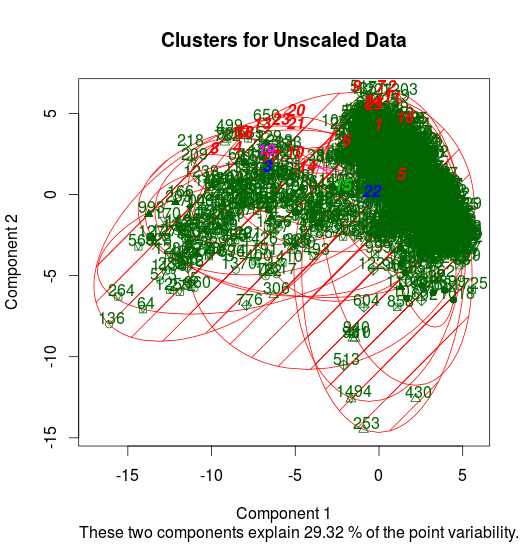
\includegraphics[scale=.435]{K_means_unscaled.png}
%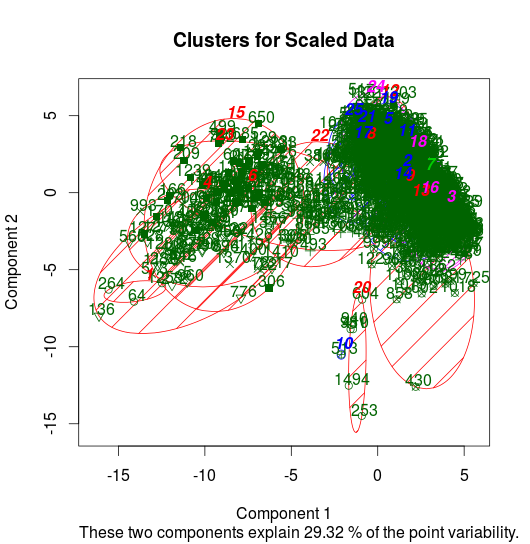
\includegraphics[scale=.435]{K_means_scaled.png}
%\end{center}

%---------------------------------------------------
%	K-MEDOIDS
%---------------------------------------------------
\subsection{K-medoids}
%K-medoids provides a similar approach to clustering as k-means, but the process relies on using a random subset of the data points to act as the middle of each cluster.  
Upon applying this approach to the test data, it becomes clear that the chosen metric influences the resulting clusters and their respective sizes.  As shown in the table below, using the Manhattan Metric, otherwise known as the $\ell_1$ metric, produces more balanced data while the Euclidean metric ($\ell_2$) partitions much of the data into fewer of the clusters.  %For example, the five largest clusters produced using the Manhattan Metric contain 521 observations while the five largest clusters under the Euclidean metric contain 753 observations.  Furthermore, using the Euclidean Metric results in 9 clusters containing a single observation whereas using the Manhattan Metric only results in 4 clusters containing a single variable.  
Considering that the Manhattan Metric produces clusters more similar in size to the true data, further exploration on the data using the Manhattan Metric might produce more desirable results.

\begin{table}[h]
\center
\caption{Cluster Sizes Produced by K-Medoids with Manhattan Metric}
\begin{tabular}{c c c c c c c c c c c c c c}
\hline
Cluster Id & 1 & 2  & 3  & 4  & 5   & 6   & 7   & 8  & 9  & 10 & 11 & 12 & 13 \\
Obs. 	   &89 & 27 & 24 & 42 & 122 & 108 & 100 & 78 & 43 & 43 & 50 & 64 & 51 \\
\hline
Cluster Id & 14 & 15  & 16 & 17 & 18 & 19 & 20 & 21 & 22 & 23 & 24 & 25 & \\
Obs.       & 29 & 102 & 46 & 1  & 19 & 51 & 2  & 1  & 2  & 4  & 1  & 1  &\\
\hline
\end{tabular}
\end{table}

%\begin{center}
%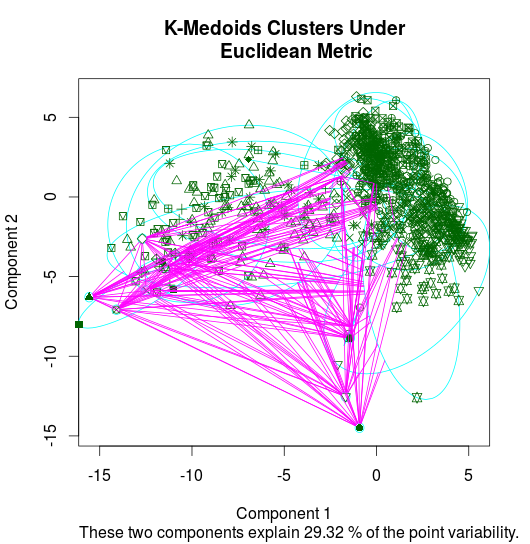
\includegraphics[scale=.435]{k_medoids_euclid.png}
%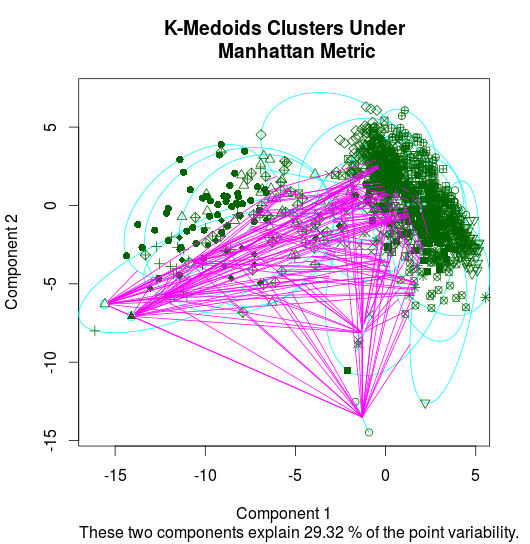
\includegraphics[scale=.435]{k_medoids_manh.png}
%\end{center}

%---------------------------------------------------
%	K-MEANS ++
%---------------------------------------------------
\subsection{K-means $++$}
K-means$++$ should provide an improved clustering result over the standard K-means approach since it thoughtfully chooses $k$ cluster centers before proceeding with the standard K-means algorithm.  Using scaled data, the five largest clusters produced with the K-means$++$ algorithm contain 635 observations: very close to the true data where the 5 largest clusters contain 623 observations.  The drawback is the large number of single or two observation clusters (6), and the significantly increased computation time.


\begin{table}[h]
\center
\caption{Cluster Sizes Produced by K-means++ }
\begin{tabular}{c c c c c c c c c c c c c c}
\hline
Cluster Id & 1  & 2 & 3 & 4  & 5   & 6  & 7 & 8 & 9   & 10 & 11  & 12  & 13 \\
Obs. 	   &124 & 1 & 1 & 33 & 170 & 21 & 7 & 2 & 111 & 9  & 105 & 104 & 63\\
\hline
Cluster Id & 14 & 15  & 16 & 17 & 18 & 19 & 20 & 21 & 22 & 23 & 24 & 25 & \\
Obs.       & 50 & 14 & 16 & 16  & 20 & 125 & 1  & 6  & 23  & 75  & 1  & 2  &\\
\hline
\end{tabular}
\end{table}

%\begin{center}
%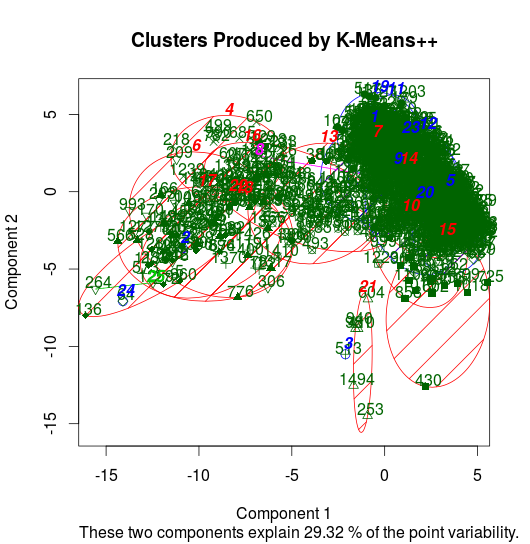
\includegraphics[scale=.435]{k_means_pp.png}
%\end{center}

%---------------------------------------------------
%	HIERARCHICAL
%---------------------------------------------------
\subsection{Hierarchical Clustering}
We consider three hierarchical clustering methods --- the ``complete," the ``single," and the ``average" linkages. Additionally, we chose to cluster on the entire training data set as well as within the three main subcategories of variable stars. Lastly, all 85 variables are normalized to the interval $[0,1]$. 

After running the normalized data through the ``complete," ``single," and ``average" linkages, we focus on analyzing the complete linkage. In essence, the single and average linkages tend to cluster a fairly sizeable amount of observations into a single cluster compared to the complete linkage. This result is further exacerbated if the explanatory variables are either left unchanged or standardized rather than normalized. For example, if the data is standardized and then clustered, cluster \#1 contains roughly 850 observation. Furthermore, this number grows to more than a thousand without standardizing. Overall, it would appear that performing the farthest-neighbors clustering on the full set of standardized variables is better able to differentiate the more ``tightly" clustered stars. Below is a table for the clusters on the non-subsetted training data as well as graphs for both subsetted and non-subsetted training data sets.

\begin{figure}[h]
	\begin{center}	
		\subfigure[All Star types ]{
		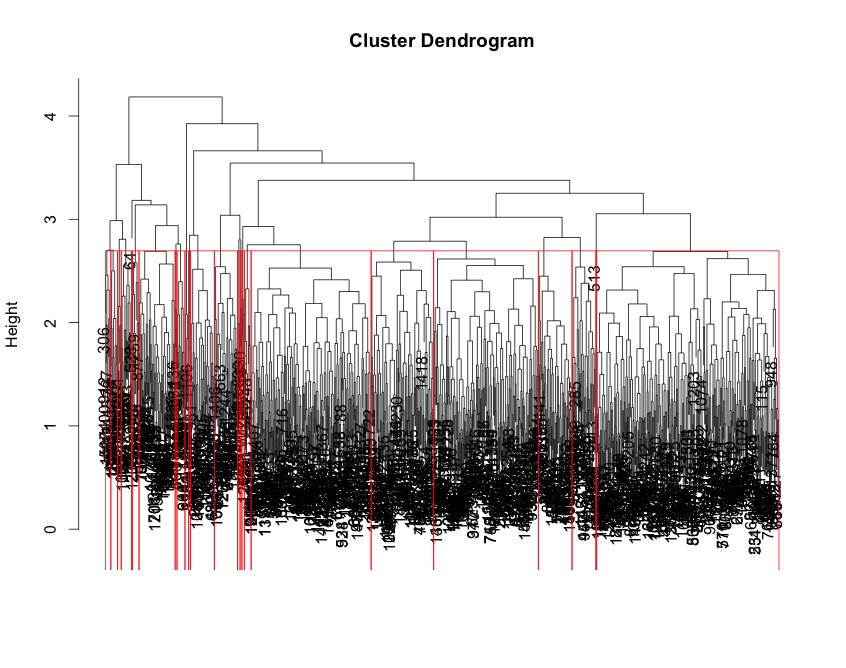
\includegraphics[scale=0.25]{dendro24group.jpeg}}
		\subfigure[Pulsating Star types only]{
		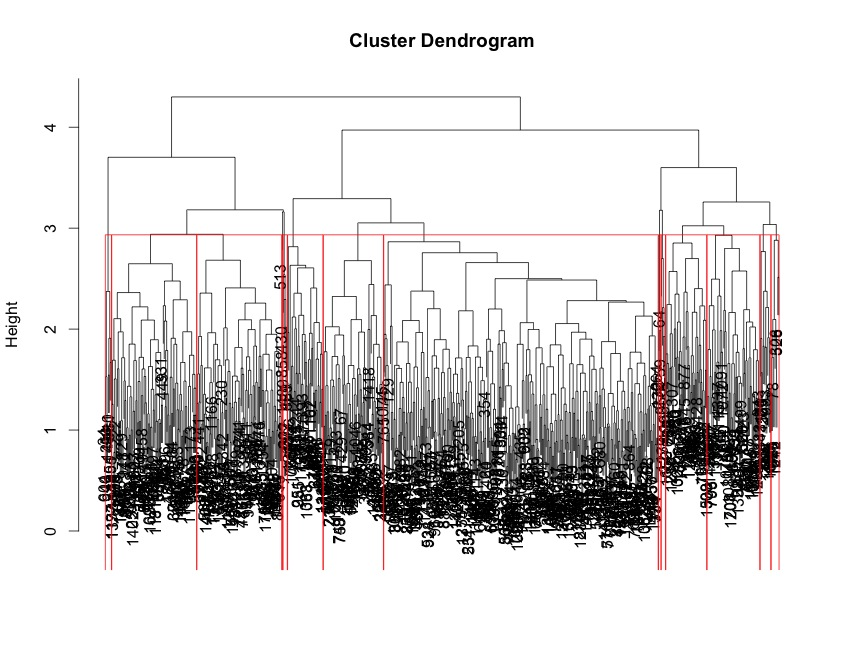
\includegraphics[scale=0.25]{dendro14group.jpeg}}  \\
		\subfigure[Eruptive Star types only]{
		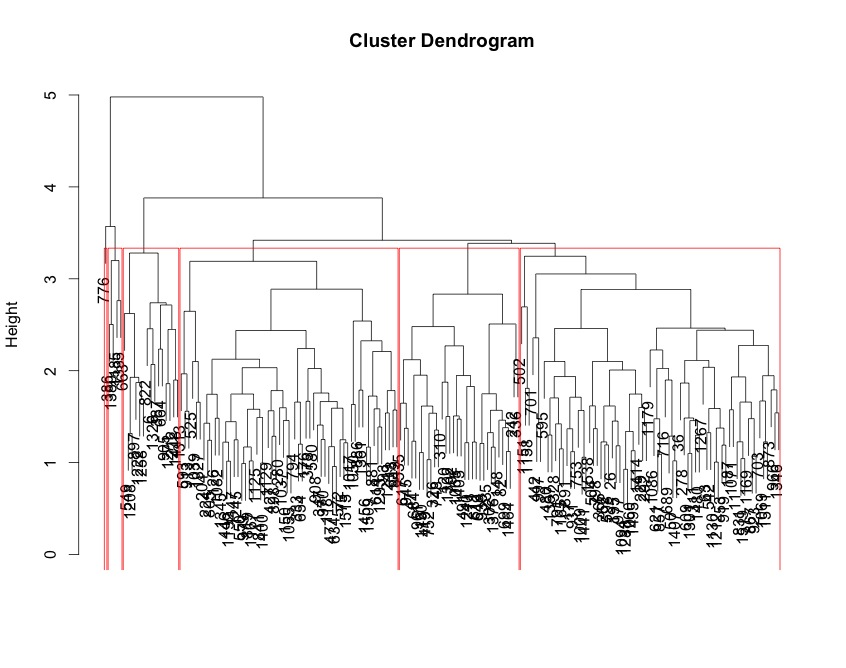
\includegraphics[scale=0.25]{dendro6group.jpeg}}
		\subfigure[Multi-Star types only]{
		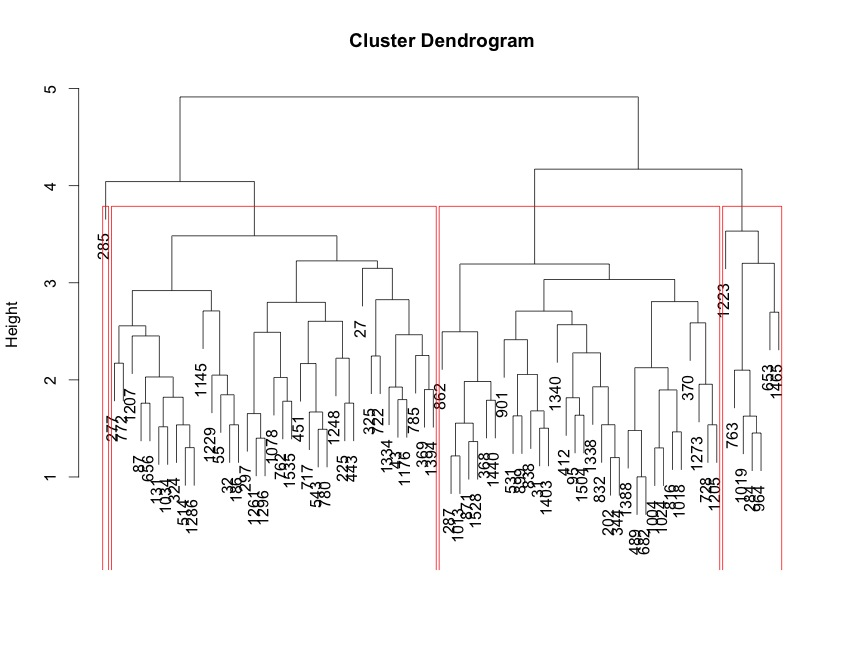
\includegraphics[scale=0.25]{dendro4group.jpeg}}
	\end{center}
\end{figure} 

\begin{table}[h]
\center
\caption{Farthest-Neighbor on Non-subsetted Training Data}
\begin{tabular}{c c c c c c c c c c c c c}
\hline
Cluster Id           & 1 & 2 & 3 & 4 & 5 & 6 & 7 & 8 & 9 & 10 & 11 & 12  \\
Obs. 		        	&196 & 59 & 11 & 171 & 298 & 102 & 39 & 9 & 38 & 39 & 55 & 1  \\
\hline
Cluster Id           & 13 & 14 & 15 & 16 & 17 & 18 & 19 & 20 & 21 & 22 & 23 & 24  \\
Obs.         		& 13 & 11 & 17 & 3 & 6 & 11 & 4 & 4 & 1 & 3 & 6 & 3  \\
\hline
\end{tabular}

\end{table}

%---------------------------------------------------
%	SPECTRAL
%---------------------------------------------------
\newpage
\subsection{Spectral Clustering}
Another method we apply is spectral clustering to determine the different clusters. For this method, we did not perform any form of dimensional reduction besides removing the covariates (around 10) that largely contained 0 entries or NAs.  
\begin{center}
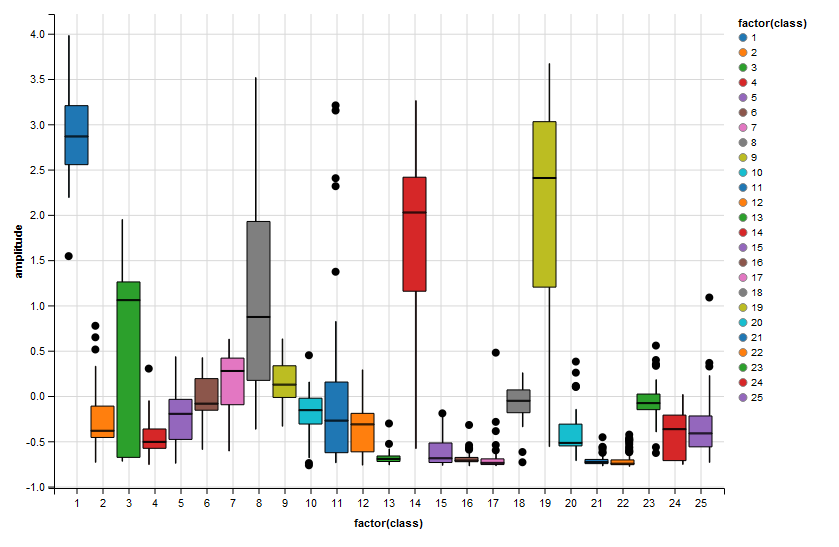
\includegraphics[scale=0.38]{estimated.png}
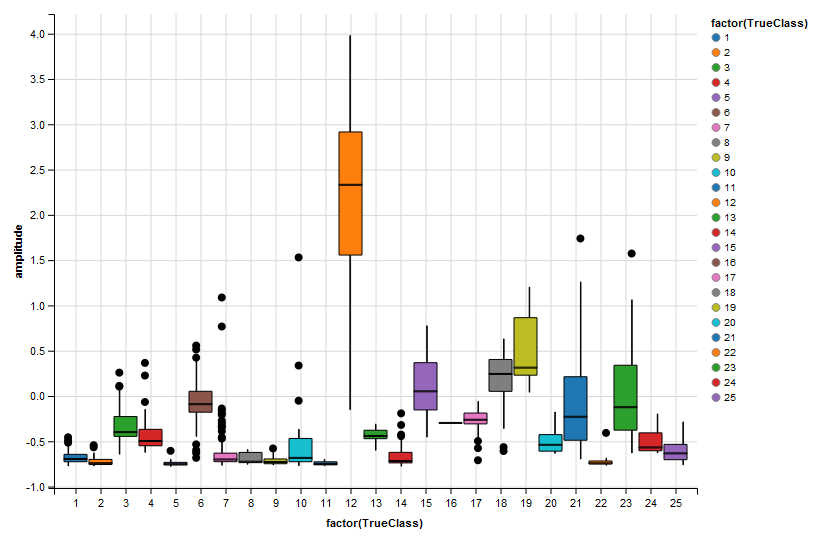
\includegraphics[scale=0.38]{trueclass.png}
\end{center}
On the left represents the estimated distribution of the clusters and on the right represents the true distribution of stars with respect to the amplitude data. 
Compared to the other methods, spectral clustering more evenly distributed the sizes between the 25 groups. An important note, the numbers along the $x$-axis do not represent the same star group as in the true classes. Instead it is the group designated by the spectral clustering. 

%---------------------------------------------------
%	FUTURE WORK
%---------------------------------------------------
\section{Discussion and Future Work}
Clustering the data proved a difficult task due to the number of variables and to the way different star classes showed variable values over similar ranges.  Even with each method considered, we would be cautious about applying these methods to actual data for fear of excessive misclassification of observations.

Future work would include further refinements to the algorithms with the goal of reducing misclassification as much as possible.  Furthermore, exploring larger data sets would likely require a reduction in the total number of variables; thus we would likely need to perform Principle Component Analysis to reduce our data to a manageable size without eliminating the components necessary for effective clustering.  
\end{document}
